\section{RepReMatch}

\subsection{Naïve Approach}
\begin{frame}{Naïve Approach}
	\begin{columns}[t, onlytextwidth]
		\begin{column}{0.6\textwidth}
			Naïve approach:
			\begin{itemize}
				\item
				repeatedly use maximum matchings

				\item
				fails because of missing foresight
				\begin{itemize}
					\item
					additive valuations:
					sort items by valuation \\
					\(\Rightarrow\) \(2n\)-approximation (SMatch)

					\item
					submodular valuations:
					lowest valuation \\
					approximable only by \(\bigomega[\big]{ \sqrt{m/\ln m} }\) \smash{\raisebox{-.25ex}{\Large\Lightning}}
				\end{itemize}
			\end{itemize}
		\end{column}
		\begin{column}{0.4\textwidth}
			\vphantom{a}\vspace{-0.5\baselineskip}\par
			\centering
			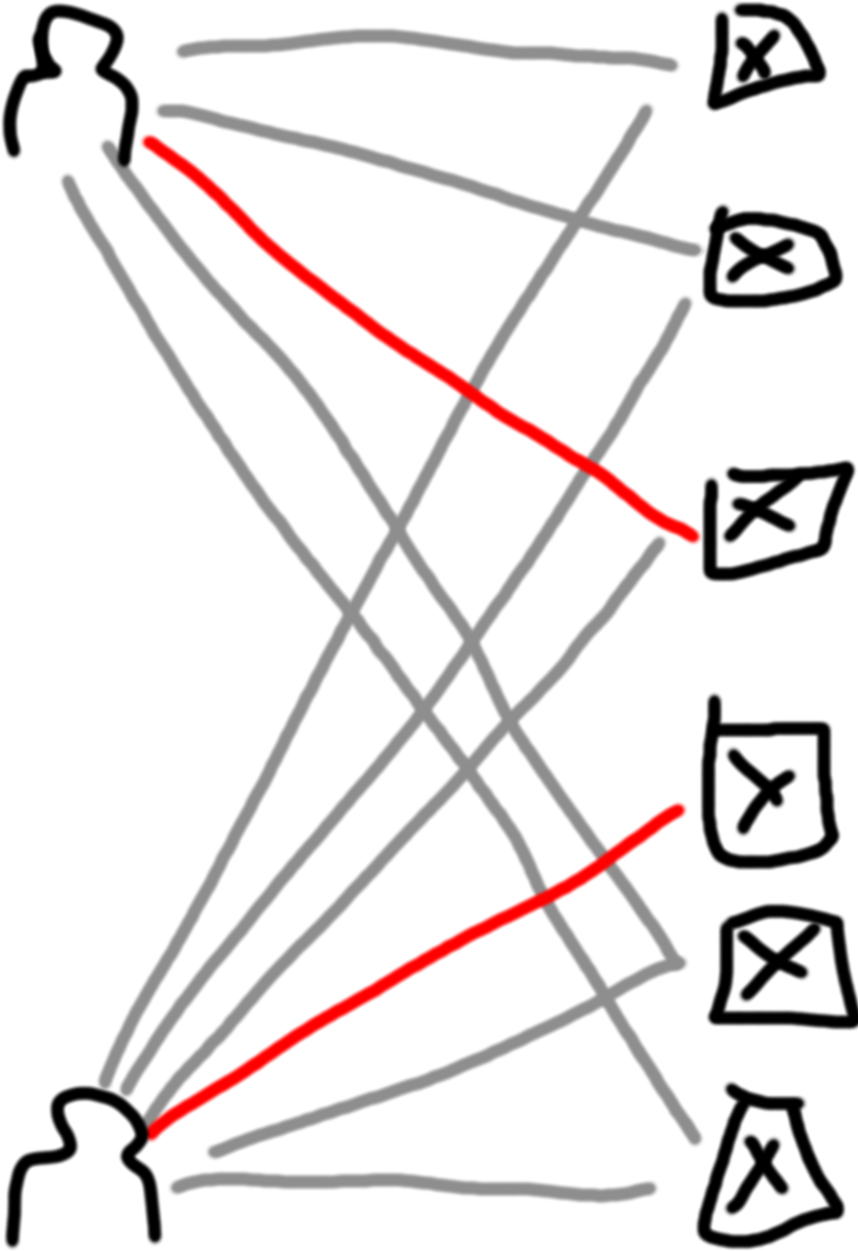
\includegraphics[height=5cm]{img/repeatedmatching}
		\end{column}
	\end{columns}
\end{frame}





\subsection{The Algorithm}
\begin{frame}{Key Ideas of the Algorithm}
	\begin{columns}[t, onlytextwidth]
		\begin{column}{0.6\textwidth}
			We need change the past in three phases:
			\begin{description}
				\item[Phase \phasei]
				Assign enough high-value items temporarily.

				\item[Phase \phaseii]
				Assign the remaining items definitely.

				\item[Phase \phaseiii]
				Re-assign the items of phase \phasei{} definitely.
			\end{description}

			\smallskip

			\begin{exampleblock}{Theorem}
				RepReMatch guarantees a \(2n(\log_2 n + 3)\)-approximation \\
				under submodular valuations.
			\end{exampleblock}
		\end{column}
		\begin{column}{0.4\textwidth}
			\vphantom{a}\vspace{-0.5\baselineskip}\par
			\centering
			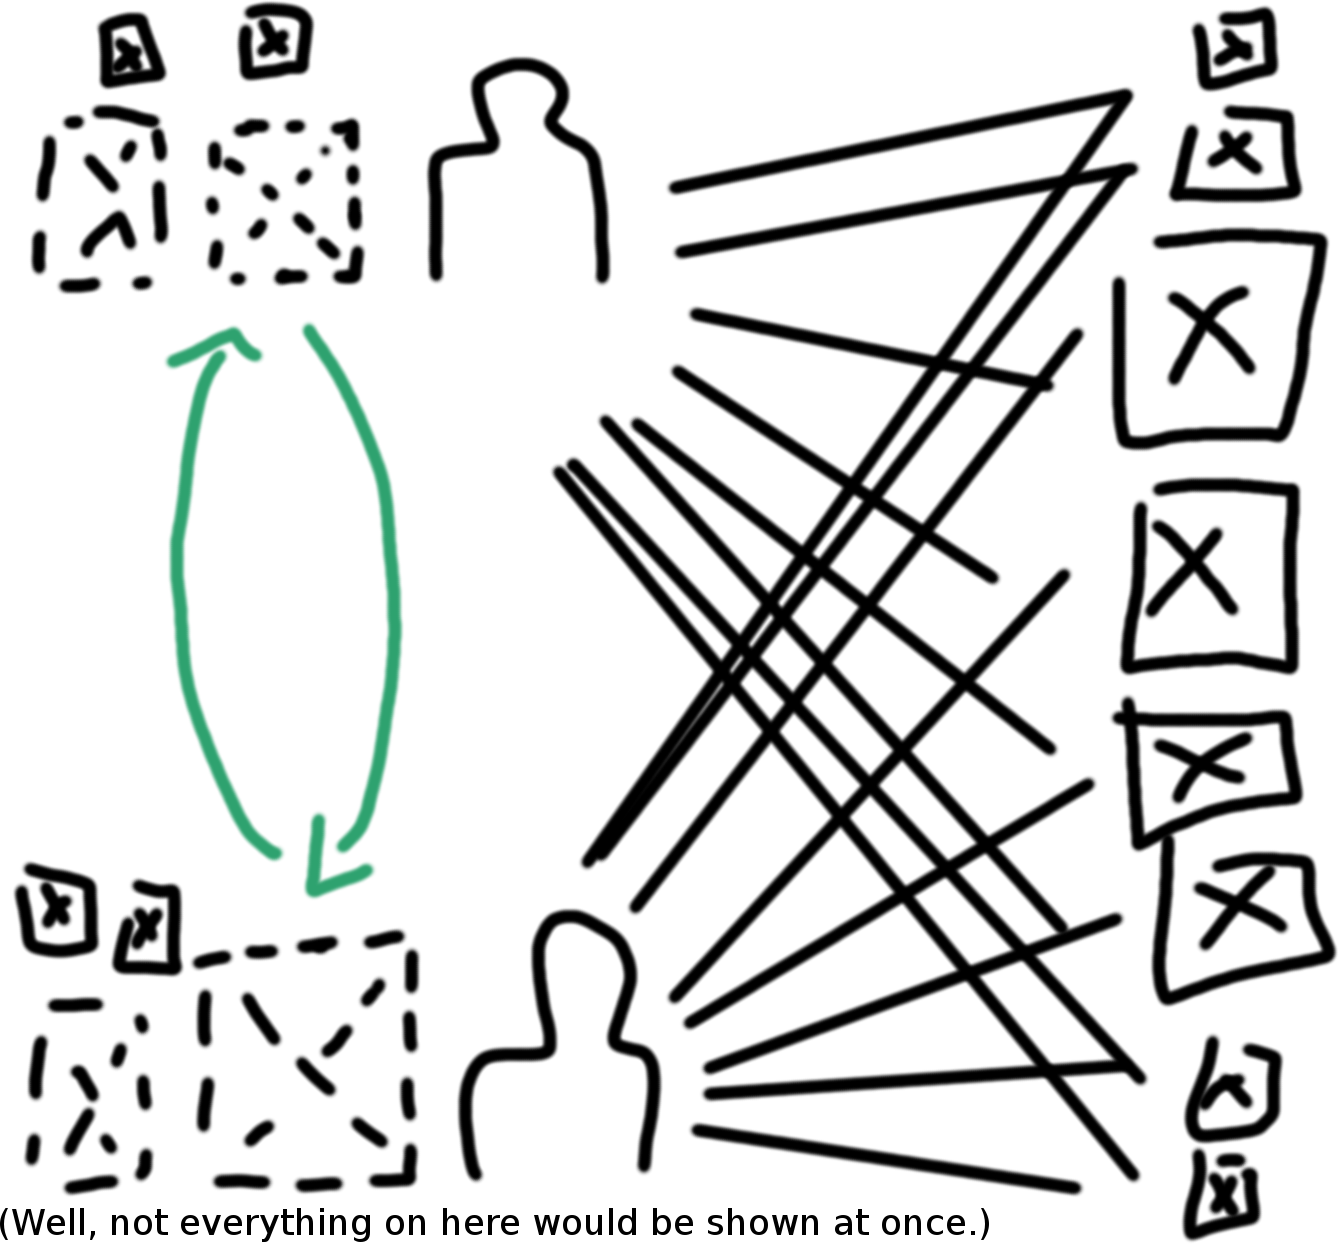
\includegraphics[height=5cm]{img/phases}
		\end{column}
	\end{columns}
\end{frame}

\begin{frame}{The Algorithm}
	Phase \phasei:
	\begin{enumerate}
		\item
		repeat \(\ceil{\log_2 n} + 1\) times
		\begin{enumerate}
			\item
			create bipartite graph \((\agents, \goods, E)\) with edge weights \(\log \valuations[ \hairspace j ]^{\weight}\)

			\item
			compute maximum weight matching

			\item
			update bundles \(\alloc[\phasei]\) \& remove assigned items
		\end{enumerate}
		\seti
	\end{enumerate}
	Phase \phaseii:
	\begin{enumerate}
		\conti
		\item
		repeat until \(\goods = \emptyset\)
		\begin{enumerate}
			\item
			create bipartite graph \((\agents, \goods, E)\) with edge weights \(\log \valuations[\alloc[\phaseii] \cup \{ \hairspace j \} ]^{\weight} \)

			\item
			compute maximum weight matching

			\item
			update bundles \(\alloc[\phaseii]\) \& remove assigned items
		\end{enumerate}
		\seti
	\end{enumerate}
	Phase \phaseiii:
	\begin{enumerate}
		\conti
		\item
		create bipartite graph \(\paren[\big]{ \agents, \bigcup_{i \in \agents} \alloc[\phasei], E }\) with edge weights \(\log \valuations[\alloc[\phaseii] \cup \{ \hairspace j \} ]^{\weight} \)

		\item
		compute maximum weight matching

		\item
		create bundles \(\alloc[\phaseiii]\)
	\end{enumerate}
\end{frame}





\subsection{Analysing Phases \texorpdfstring{\phasei{} \& \phaseiii}{I \& III}}
\begin{frame}{Analysing Phases \phasei{} \& \phaseiii{} (1/2)}
	Phase \phasei{} reserves \enquote{high-value} items.
	But what qualifies as \enquote{high-value}?

	\begin{definition}
		Let \(\alloc* = \braces[\big]{ \asgd*{1}, \asgd*{2}, \dots }\) be an optimal bundle.
		An item \(\genericitem \in \goods\) is \emph{outstanding} if \(\valuations[ \hairspace \genericitem] \ge \valuations[\asgd*{1}][\big]\).
	\end{definition}

	\(\Rightarrow\) Are enough outstanding items reserved?
\end{frame}

\begin{frame}{Analysing Phases \phasei{} \& \phaseiii{} (2/2)}
	\adjustfortopblock
	\begin{lemma}
		Each agent can be matched with an outstanding item in phase \phaseiii.
	\end{lemma}
	\begin{columns}[T]
		\begin{column}{0.6\textwidth}
			\begin{itemize}
				\item
				maximum number of unmatched agents halved \\
				with each round of phase \phasei
				\begin{itemize}
					\item
					\(\ceil{\log_2 n} + 1\) rounds in phase \phasei{} are enough
				\end{itemize}

				\item
				induction on number of rounds in phase \phasei
			\end{itemize}
			Base Case: In round \(1\) of phase \phasei, either
			\begin{itemize}
				\item
				\(\ge n/2\) many agents matched with an outstanding item

				\item
				\(< n/2\) many agents matched with an outstanding item
				\begin{itemize}
					\item
					\(> n/2\) many items \(\asgd*{1}\) assigned to someone else

					\item
					\(> n/2\) many agents matched upon release in phase \phaseiii
				\end{itemize}
			\end{itemize}
		\end{column}
		\begin{column}{0.375\textwidth}
			\centering
			\begin{tikzpicture}
				\node at (0, 0) {
\includegraphics[height=7mm]{img/outstanding_agent}};
				\node at (0, 1) {
\includegraphics[height=7mm]{img/outstanding_agent}};
				\node at (0, 2) {
\includegraphics[height=7mm]{img/outstanding_agent}};
				\node at (0, 3) {
\includegraphics[height=7mm]{img/outstanding_agent}};
				\node at (0, 4) {
\includegraphics[height=7mm]{img/outstanding_agent}};
			\end{tikzpicture}
%			\includegraphics<1>[height=4.25cm]{img/outstanding_1}%
%			\includegraphics<2>[height=4.25cm]{img/outstanding_2}%
%			\includegraphics<3>[height=4.25cm]{img/outstanding_3}%
%			\includegraphics<4>[height=4.25cm]{img/outstanding_4}%
		\end{column}
	\end{columns}
\end{frame}





\subsection{Analysing Phase \texorpdfstring{\phaseii}{II}}
\begin{frame}[fragile]{Analysing Phase \phaseii{} (1/2)}
	\adjustfortopblockincolumn
	\begin{columns}[t, onlytextwidth]
		\begin{column}{0.55\textwidth}
			\begin{definition}<2->
				The set \(\lostset{r}\) of \emph{lost items} is the set of all optimal items \(j \in \alloc*\)
				\onslide<3->{assigned to other agents \(i' \neq i\) in round \(r\).}
			\end{definition}
			\begin{definition}<4->
				Let \(\alloc[\phaseii] = \braces[\big]{ \asgd{1}, \asgd{2}, \dots }\) be the bundle of agent \(i\).
				\onslide<5->{The set of \emph{optimal and attainable items} is defined as
				\begin{equation*}
					\attopt{r} \coloneq \begin{cases*}
						\onslide*<-10>{\phantom}{\alloc* \setminus \paren[\big]{ \bigcup_{i' \in \agents} \alloc[\phasei][i'] \cup \lostset{1} }}
						& \onslide*<-5>{\phantom}{in round \(r = 1\), } \\
						\onslide*<-18>{\phantom}{ \attopt{r-1} \setminus \paren[\big]{ \lostset{r} \cup \braces[\big]{ \asgd{r-1} } } }
						& \onslide*<-11>{\phantom}{in round \(r \ge 2\).}
					\end{cases*}
				\end{equation*}}
			\end{definition}

			\onslide<20->{\(\Rightarrow\) What is the valuation of the remaining items?}
		\end{column}
		\begin{column}{0.45\textwidth}
			\begin{figure}
				\begin{tikzpicture}
					\node< 7- 9> {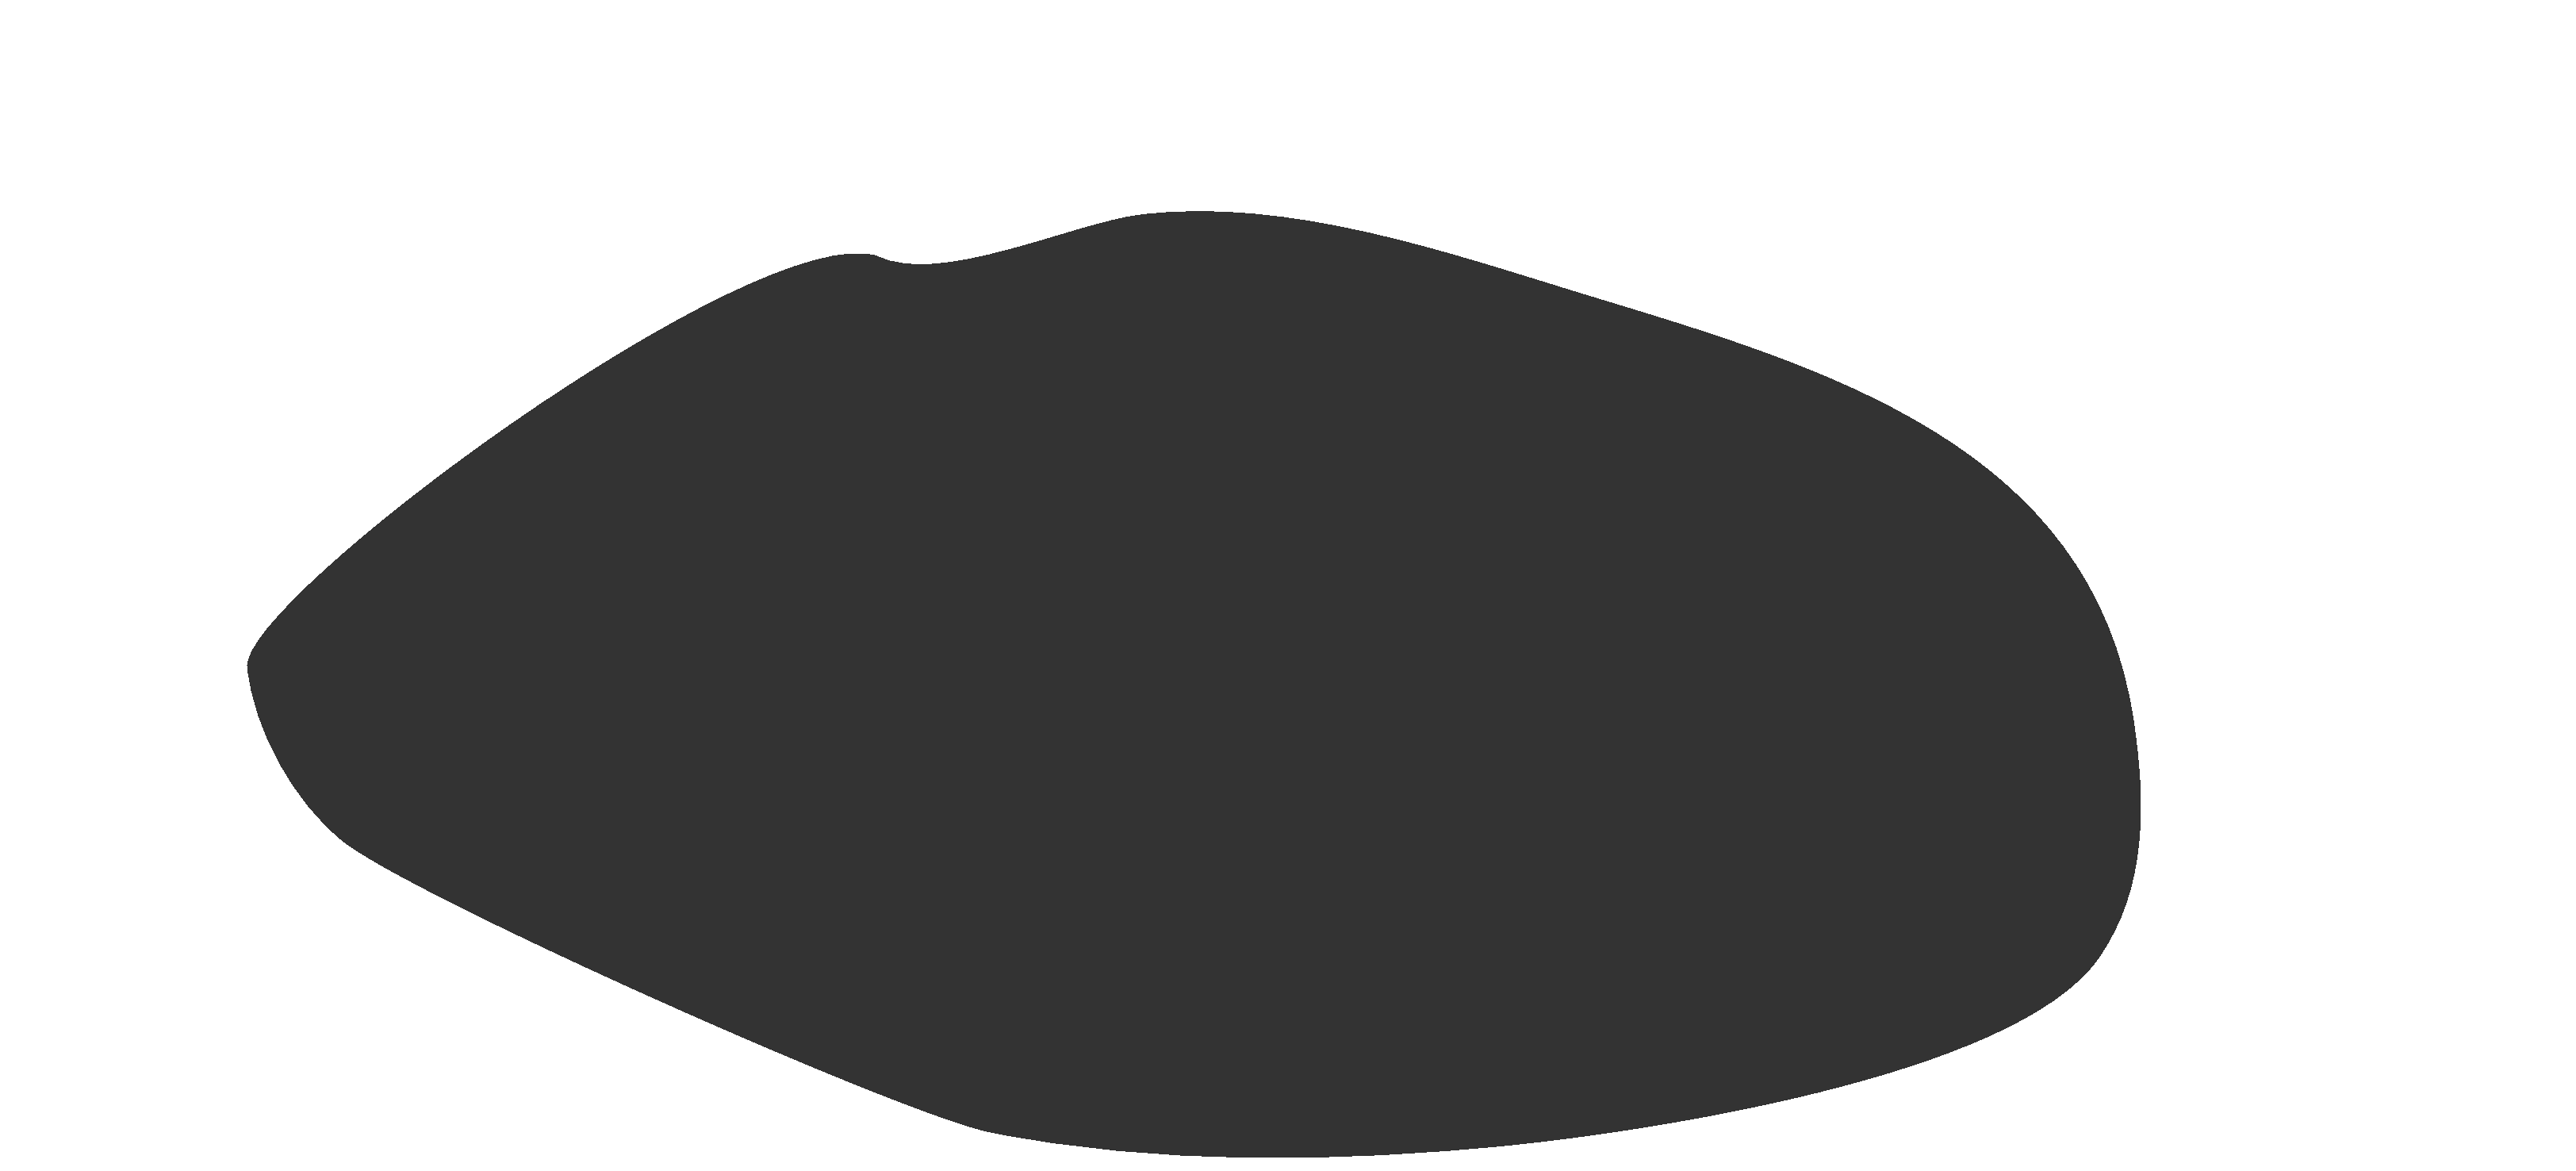
\includegraphics[height=25mm]{optainable_r1_optblack}};
					\node<10-  > {
\includegraphics[height=25mm]{optainable_r1_optgrey}};
					\node< 8-  > {
\includegraphics[height=25mm]{optainable_r1_phIfill}};
					\node< 7-  > {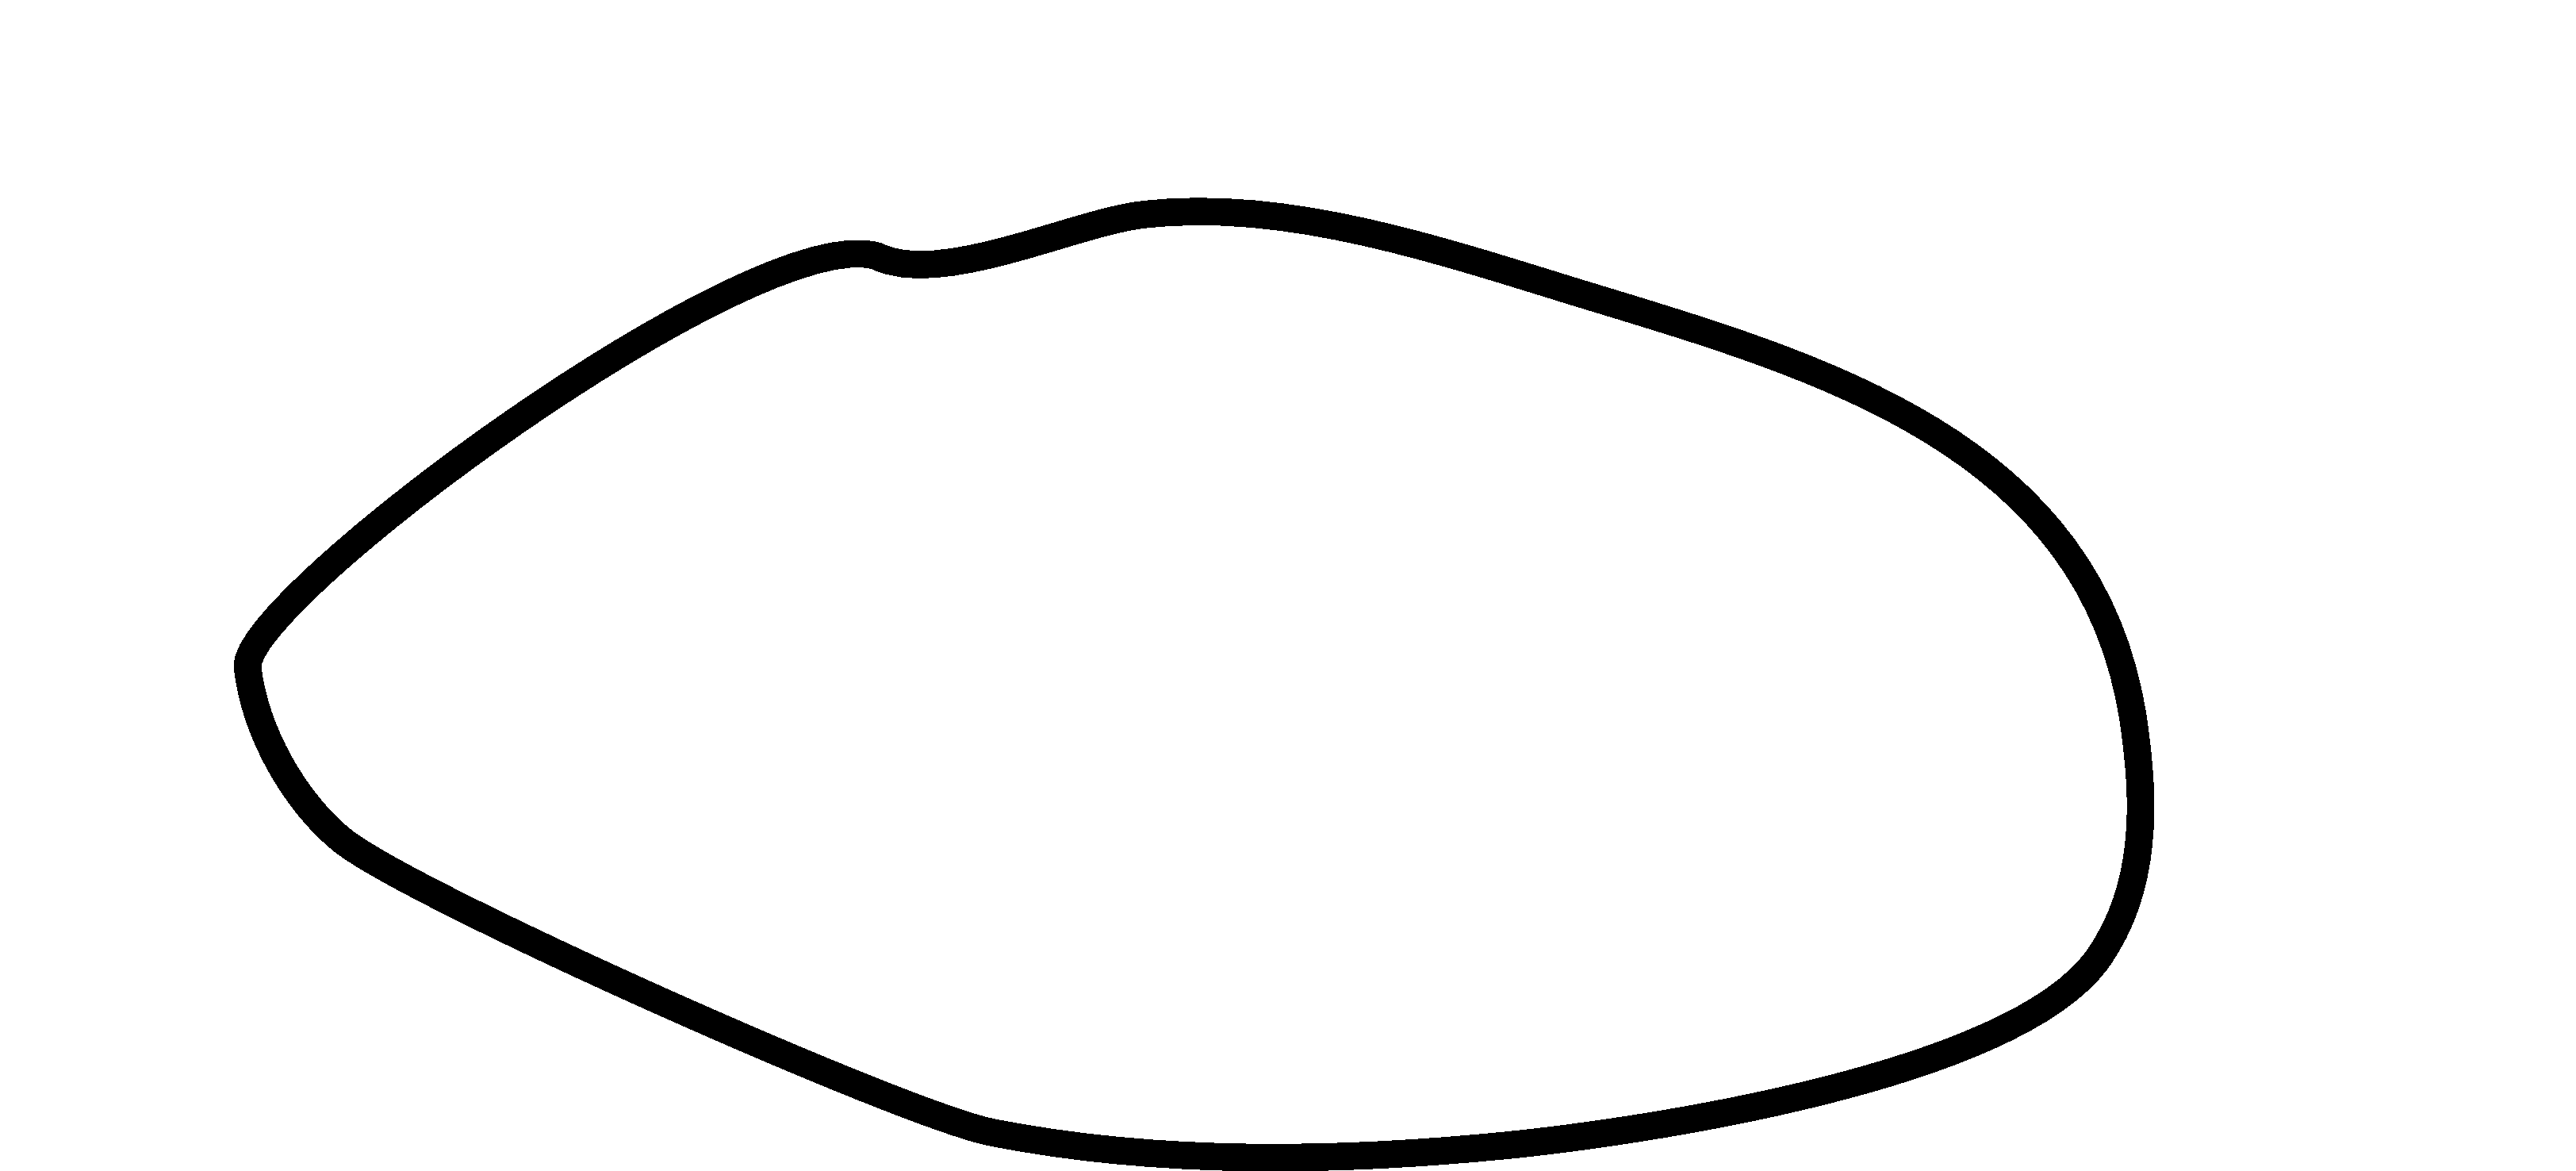
\includegraphics[height=25mm]{optainable_r1_optoutline}};
					\node< 8-  > {
\includegraphics[height=25mm]{optainable_r1_phIoutline}};
					\node< 9-  > {
\includegraphics[height=25mm]{optainable_r1_lost}};

					\node< 7->[legend            ] at (-2.00,  0.50) {\(\alloc*\)};
					\node< 8->[legend, emorot    ] at ( 2.00,  0.65) {\(\bigcup_{i' \in \agents} \alloc[\phasei][i']\)};
					\node< 9->[legend, goetheblau] at (-0.65,  0.25) {\(\lostset{1}\)};
					\node<10->[legend, dunkelgrau] at (-0.30, -0.75) {\(\attopt{1}\)};
				\end{tikzpicture}

				\vspace{2ex}

				\let\asgd\asgdbf
				\begin{tikzpicture}
					\node<13-17> {
\includegraphics[height=25mm]{optainable_r2_optblack}};
					\node<18-  > {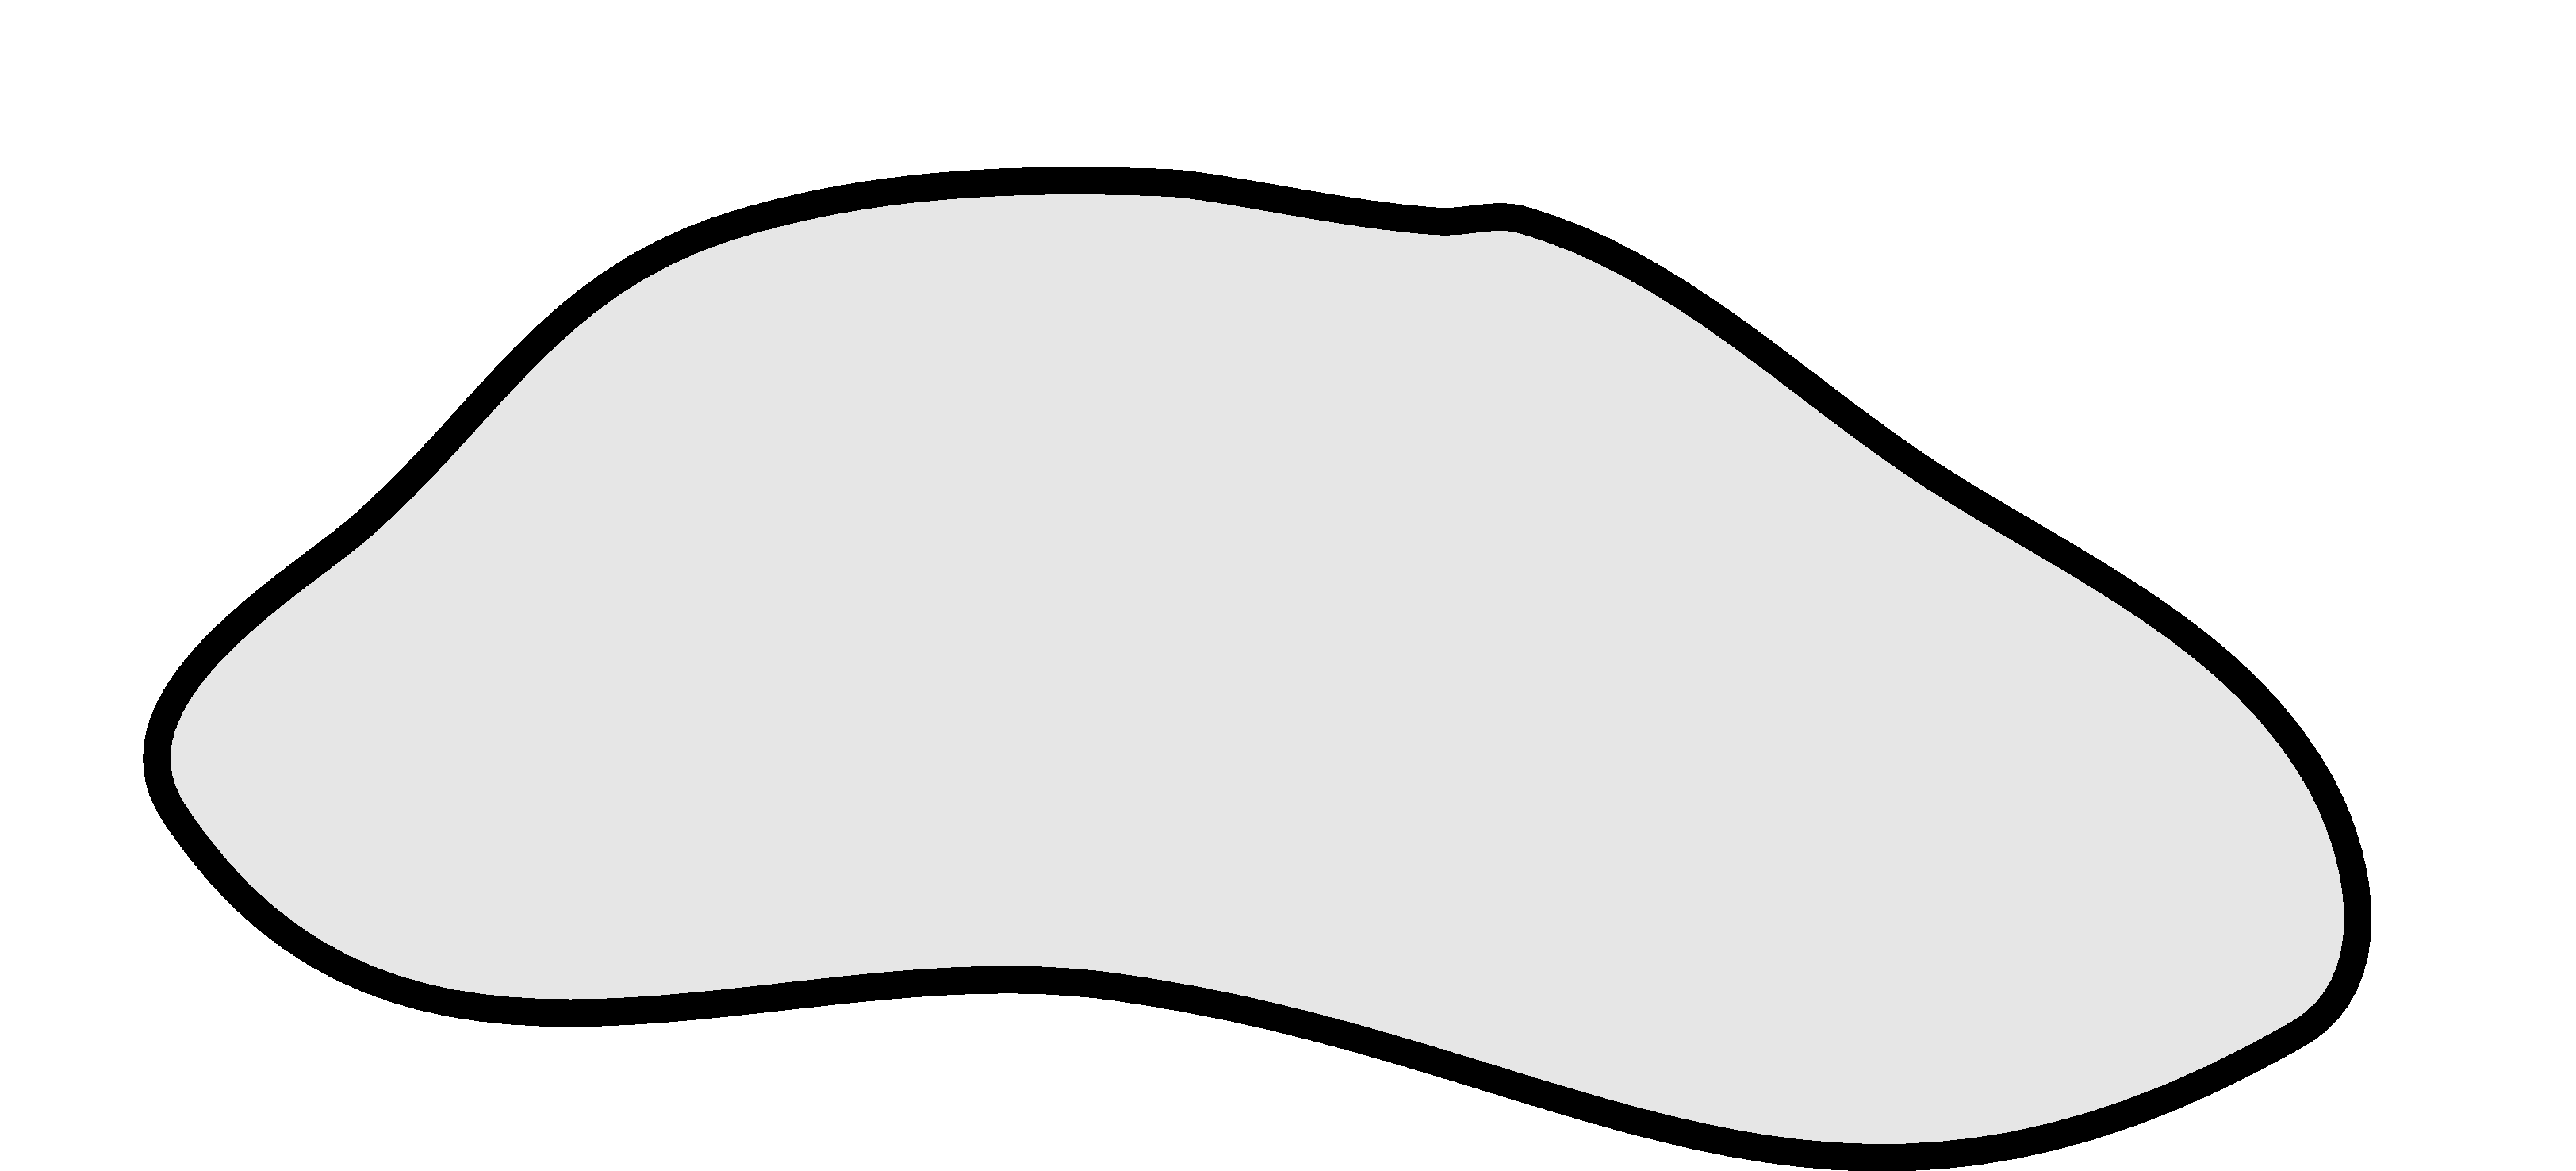
\includegraphics[height=25mm]{optainable_r2_optgrey}};
					\node<14-  > {
\includegraphics[height=25mm]{optainable_r2_lost}};
					\node<16-  > {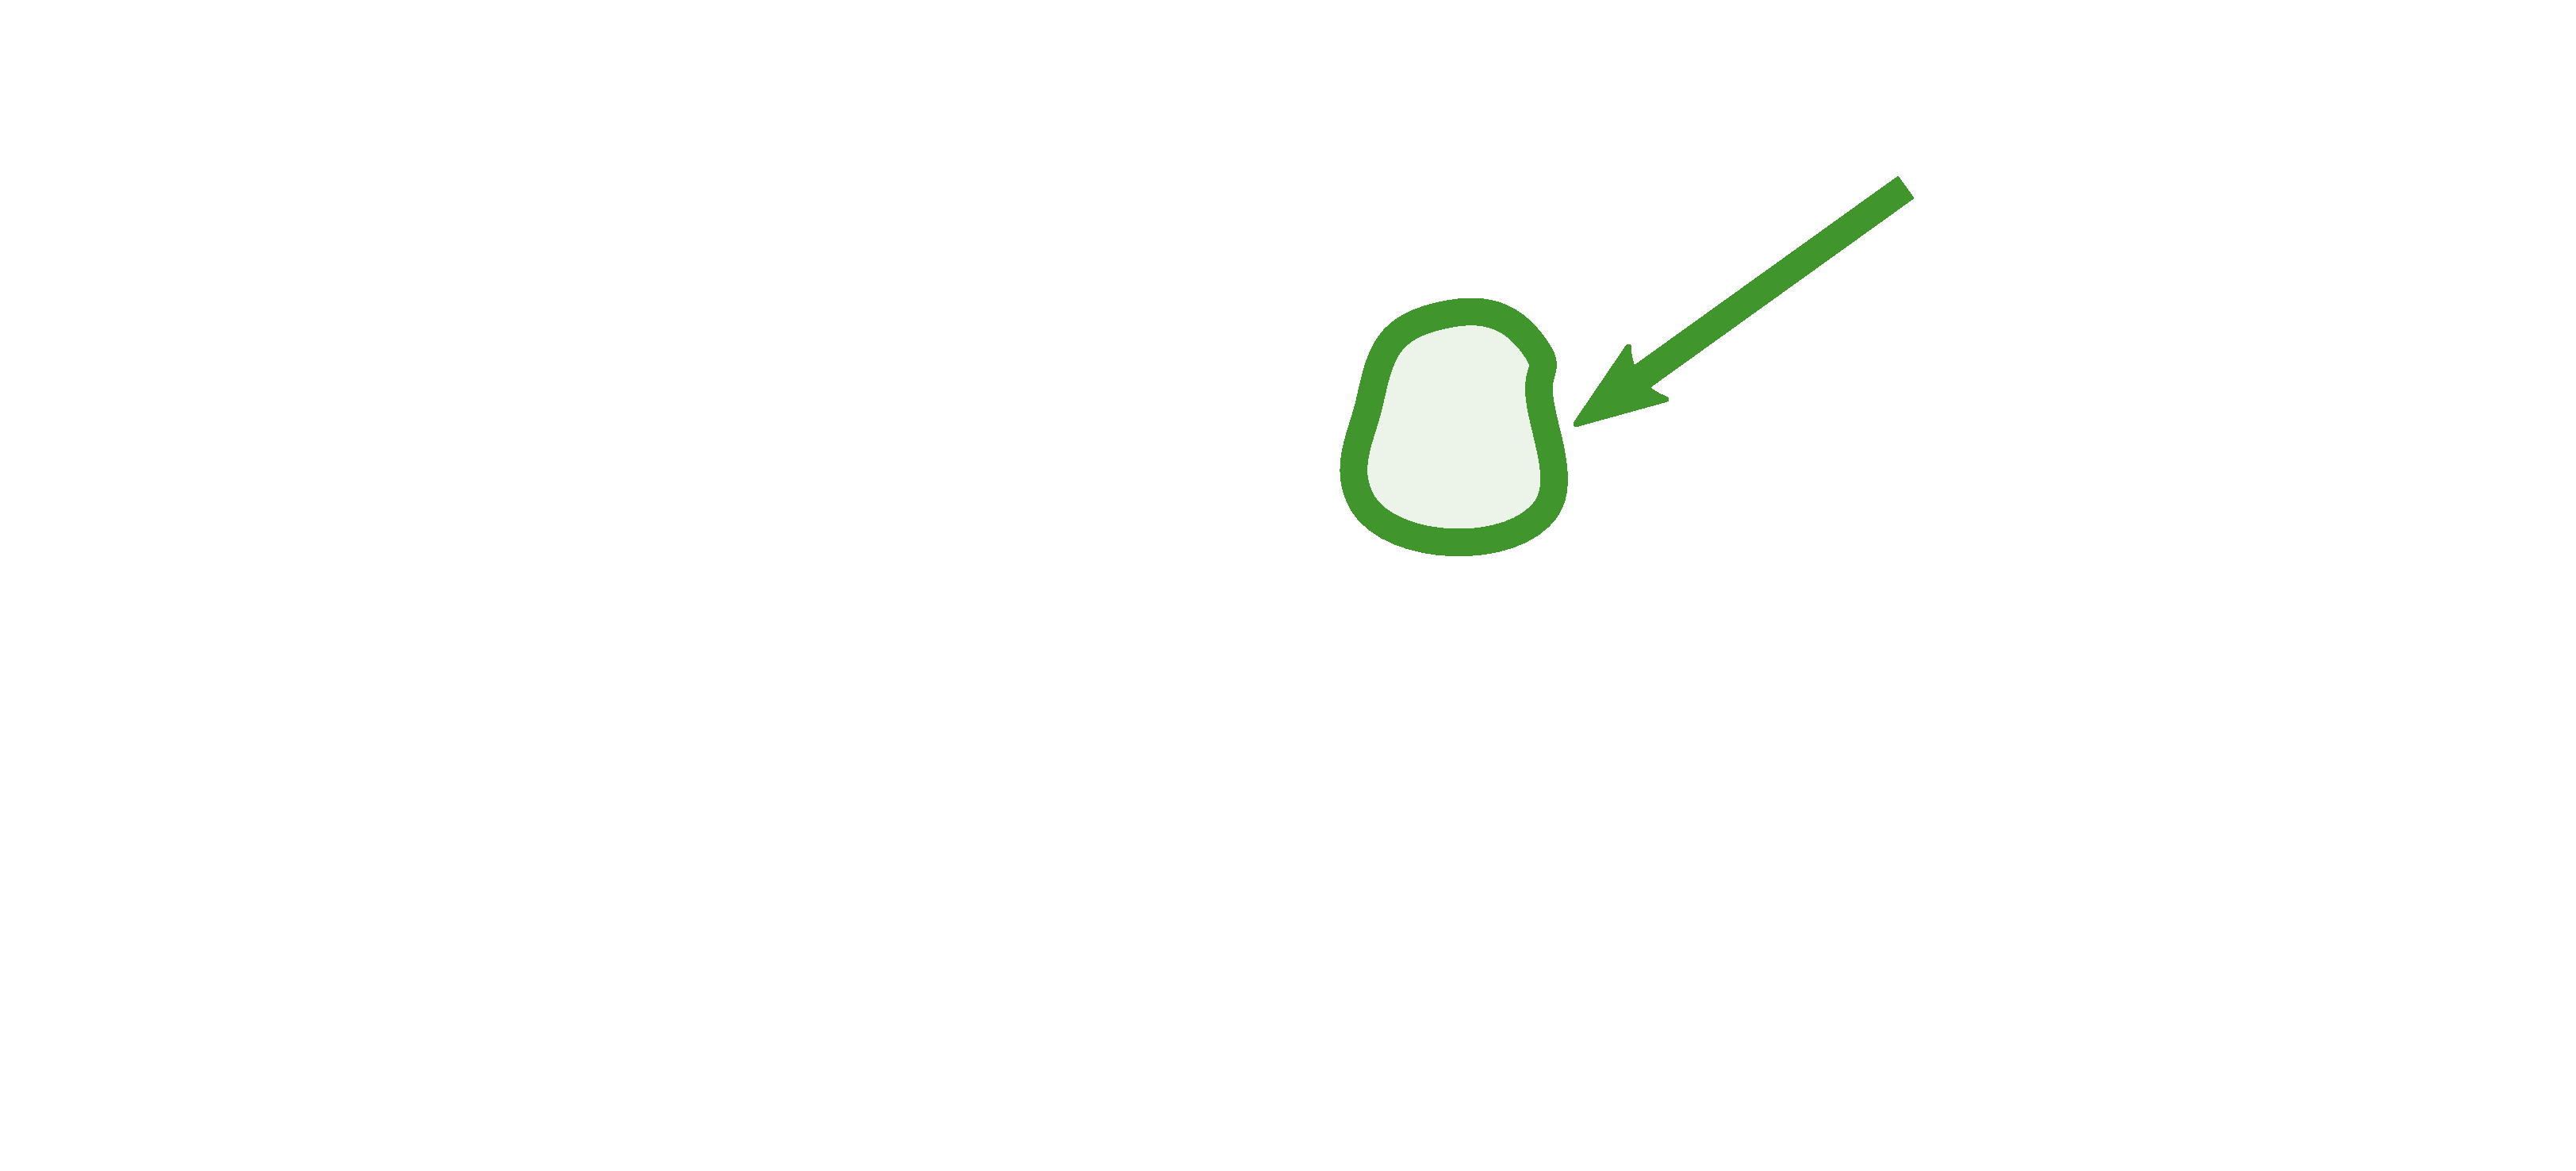
\includegraphics[height=25mm]{optainable_r2_asgdleft}};
					\node<17-  > {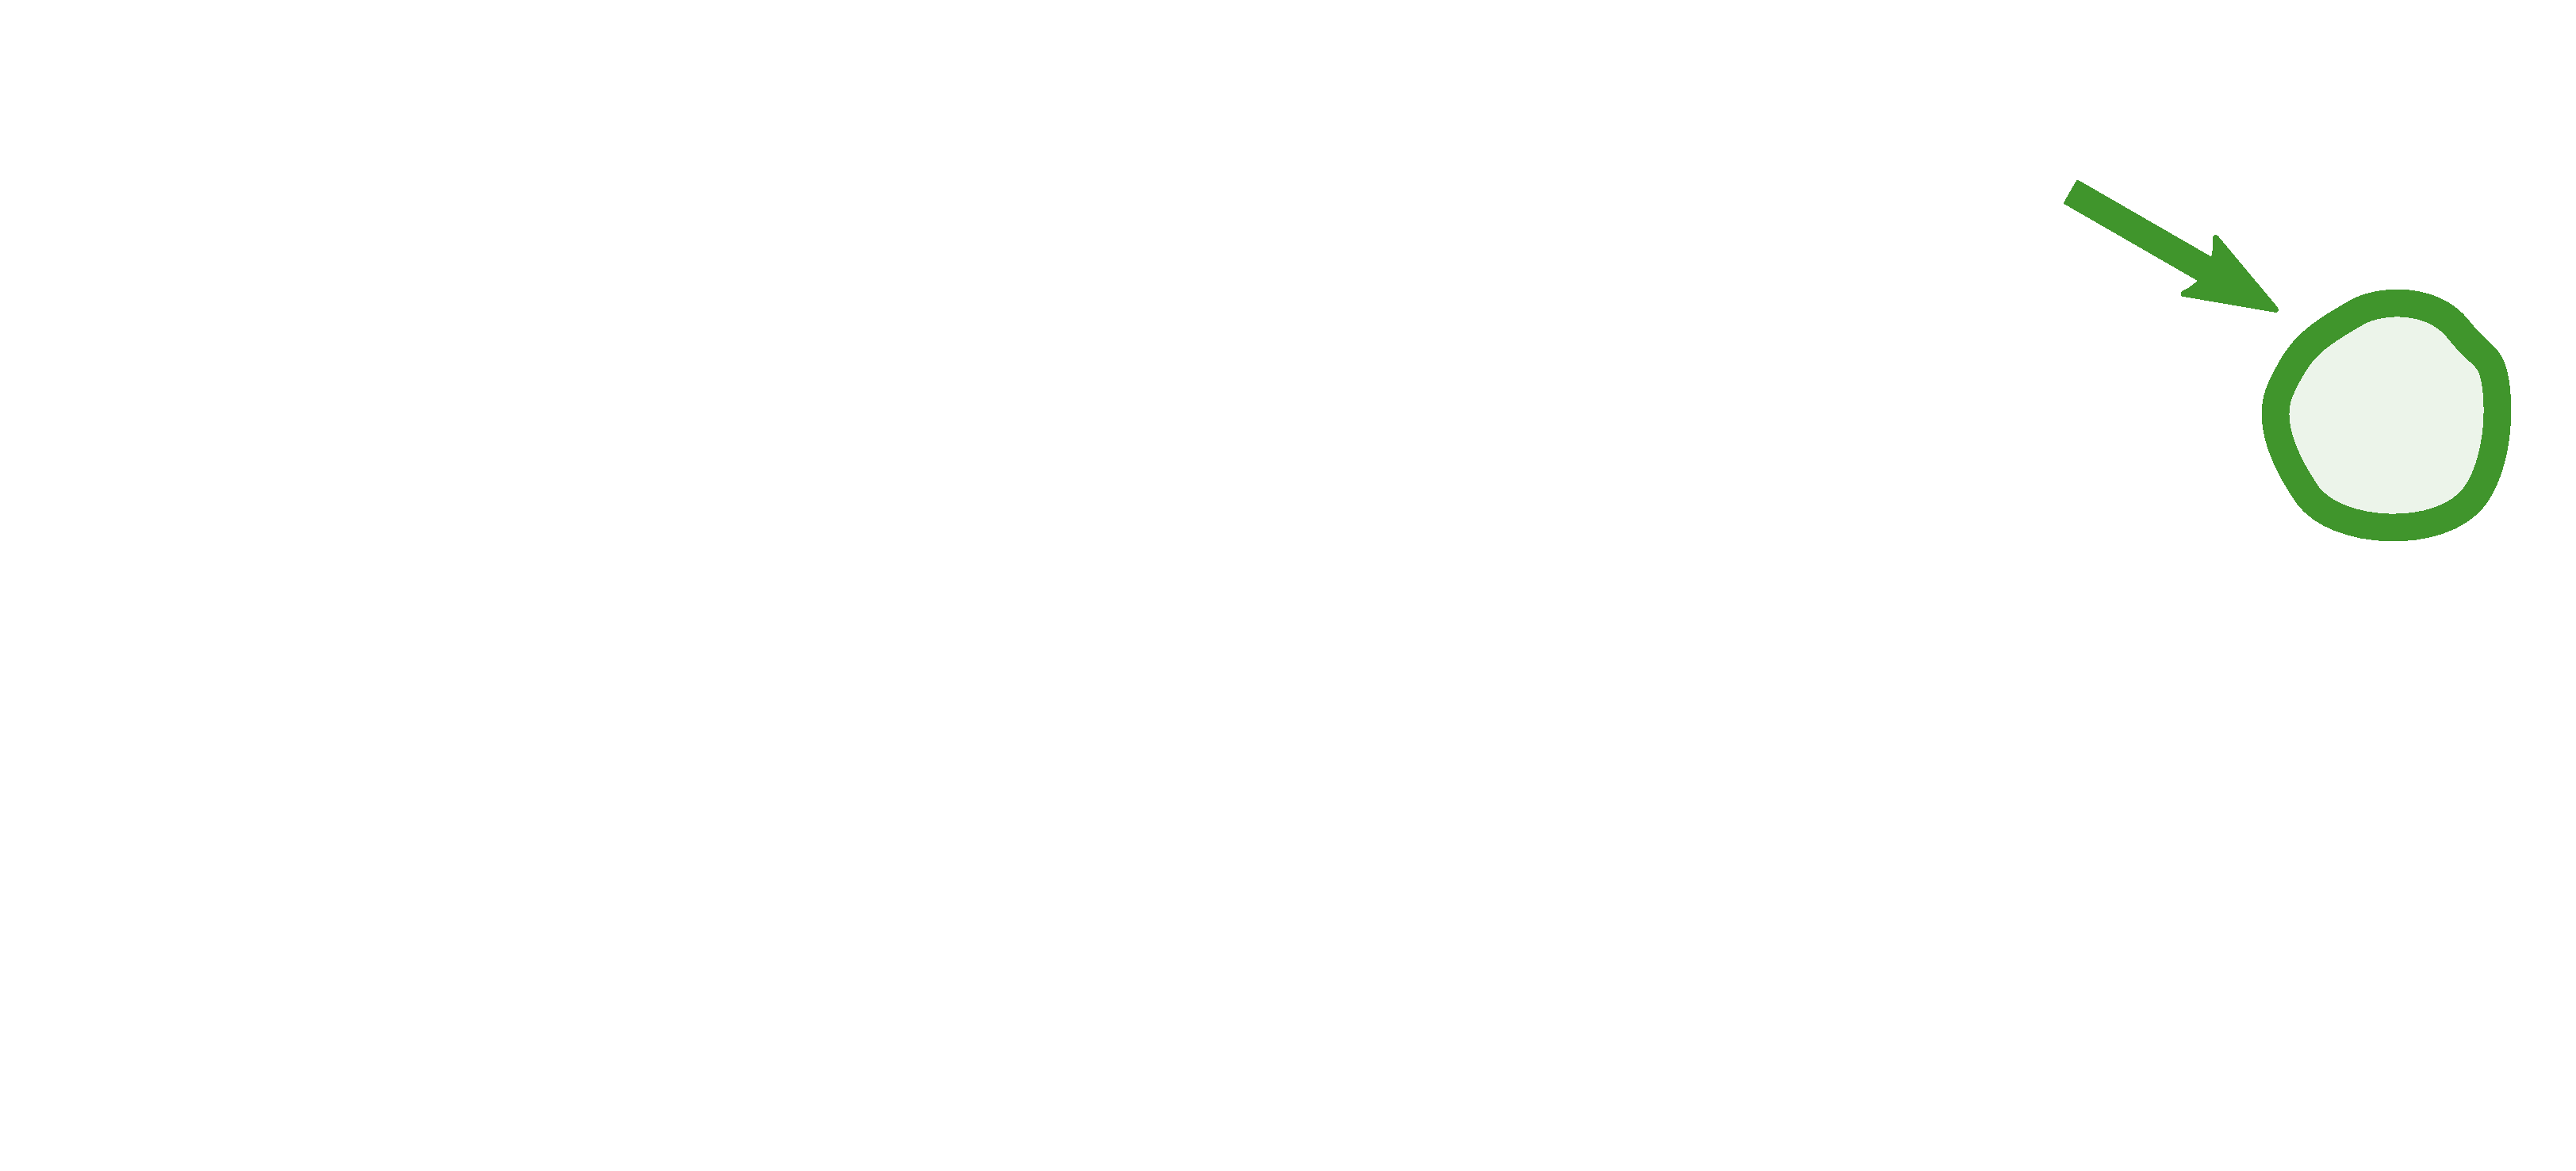
\includegraphics[height=25mm]{optainable_r2_asgdright}};
					\node<18-  > {
\includegraphics[height=25mm]{optainable_r2_optoverlay}};

					\node<13->[legend             ] at (-2.15,  0.75) {\(\attopt{r-1}\)};
					\node<14->[legend, goetheblau ] at ( 1.75, -0.65) {\(\lostset{1}\)};
					\node<15->[legend, dunkelgruen] at ( 1.67,  1.00) {\(\asgd{r-1}\)};
					\node<16->[legend, dunkelgruen] at ( 0.36,  0.35) {\(?\)};
					\node<17->[legend, dunkelgruen] at ( 2.35,  0.35) {\(?\)};
					\node<18->[legend, dunkelgrau ] at (-0.75, -0.25) {\(\attopt{r}\)};
				\end{tikzpicture}
			\end{figure}
		\end{column}
	\end{columns}
\end{frame}

\begin{frame}{Analysing Phase \phaseii{} (2/2)}
	\adjustfortopblock
	\begin{lemma}<2->
		\vspace{-3ex}
		\begin{flalign*}
			\valuations[ \attopt{r} \given \asgd{1}, \dots, \asgd{r-1} ][\big]
			\temporal<19-24>{}{=}{\ge}
			\onslide*<19-20>{\valuations[ \attopt{r} \cup \braces[\big]{\asgd{1}, \dots, \asgd{r-1}} ][\big] \alertmath<20>{{} - \valuations[\asgd{1}, \dots, \asgd{r-1}][\big]}}
			\onslide*<21-  >{\alertmath<21>{- \valuations[\asgd{1}, \dots, \asgd{r-1}][\big]} +}
			\onslide*<21-24>{\alertmath<22-24>{\valuations[ \attopt{r} \cup \braces[\big]{\asgd{1}, \dots, \asgd{r-1}} ][\big]}}
			\onslide*<25-  >{\valuations[ \attopt{1} ][\big]}
			\onslide*<26-28>{- \valuations[ \lostset{2} \given \asgd{1} ][\big]}
			\onslide*<27-28>{- \valuations[ \lostset{3} \given \asgd{1}, \asgd{2} ][\big]}
			\onslide*<28   >{- \dots}
			\onslide*<29-37>{- \!\!\sum_{l=2}^{r} \valuations[ \lostset{l} \given \asgd{1}, \dots, \asgd{l-1} ][\big] }
			\onslide*<38-40>{- \!\!\sum_{l=2}^{r} \smashoperator[r]{\sum_{\genericitem \in \lostset{l}}} \valuations[ \hairspace\genericitem \given \asgd{1}, \dots, \alertmath<40>{\asgd{l-1}} ][\big] }
			\onslide*<41-42>{- \!\!\sum_{l=2}^{r} \smashoperator[r]{\sum_{\genericitem \in \lostset{l}}} \valuations[ \hairspace\genericitem \given \asgd{1}, \dots, \alertmath<41>{\asgd{l-2}} ][\big] }
			\onslide*<43   >{- \!\!\sum_{l=2}^{r} \smashoperator[r]{\sum_{\genericitem \in \lostset{l}}} \valuations[ \asgd{l-1} \given \asgd{1}, \dots, \asgd{l-2} ][\big] }
			\onslide*<44   >{- \!\!\sum_{l=2}^{r} \abs{\lostset{l}} \cdot \valuations[ \asgd{l-1} \given \asgd{1}, \dots, \asgd{l-2} ][\big] }
			\onslide*<45   >{- \!\!\sum_{l=2}^{r} (n-1) \cdot \valuations[ \asgd{l-1} \given \asgd{1}, \dots, \asgd{l-2} ][\big] }
			\vphantom{\sum_{\genericitem \in \lostset{l}}^{r}}&&
		\end{flalign*}
	\end{lemma}
	\vspace{-1ex}
	\begin{figure}
		\hspace{-3em}
		\begin{tikzpicture}
			\node<  - 2>[opacity=0] {
\includegraphics[height=45mm]{optainable_anal_asgdf_1}};  % prevents wobbling of lemma block in otherwise empty page
			\node< 3-  > {
\includegraphics[height=45mm]{optainable_anal_optblack}};
			\node<18-  > {
\includegraphics[height=45mm]{optainable_anal_optgrey}};
			\node< 4- 5> {
\includegraphics[height=45mm]{optainable_anal_asgdf_1}};
			\node< 6- 7> {
\includegraphics[height=45mm]{optainable_anal_asgdf_2}};
			\node< 8- 9> {
\includegraphics[height=45mm]{optainable_anal_asgdf_3}};
			\node<10-11> {
\includegraphics[height=45mm]{optainable_anal_asgdf_4}};
			\node<12-13> {
\includegraphics[height=45mm]{optainable_anal_asgdf_5}};
			\node<14-15> {
\includegraphics[height=45mm]{optainable_anal_asgdf_6}};
			\node<16-  > {
\includegraphics[height=45mm]{optainable_anal_asgdf_7}};
			\node< 3-  > {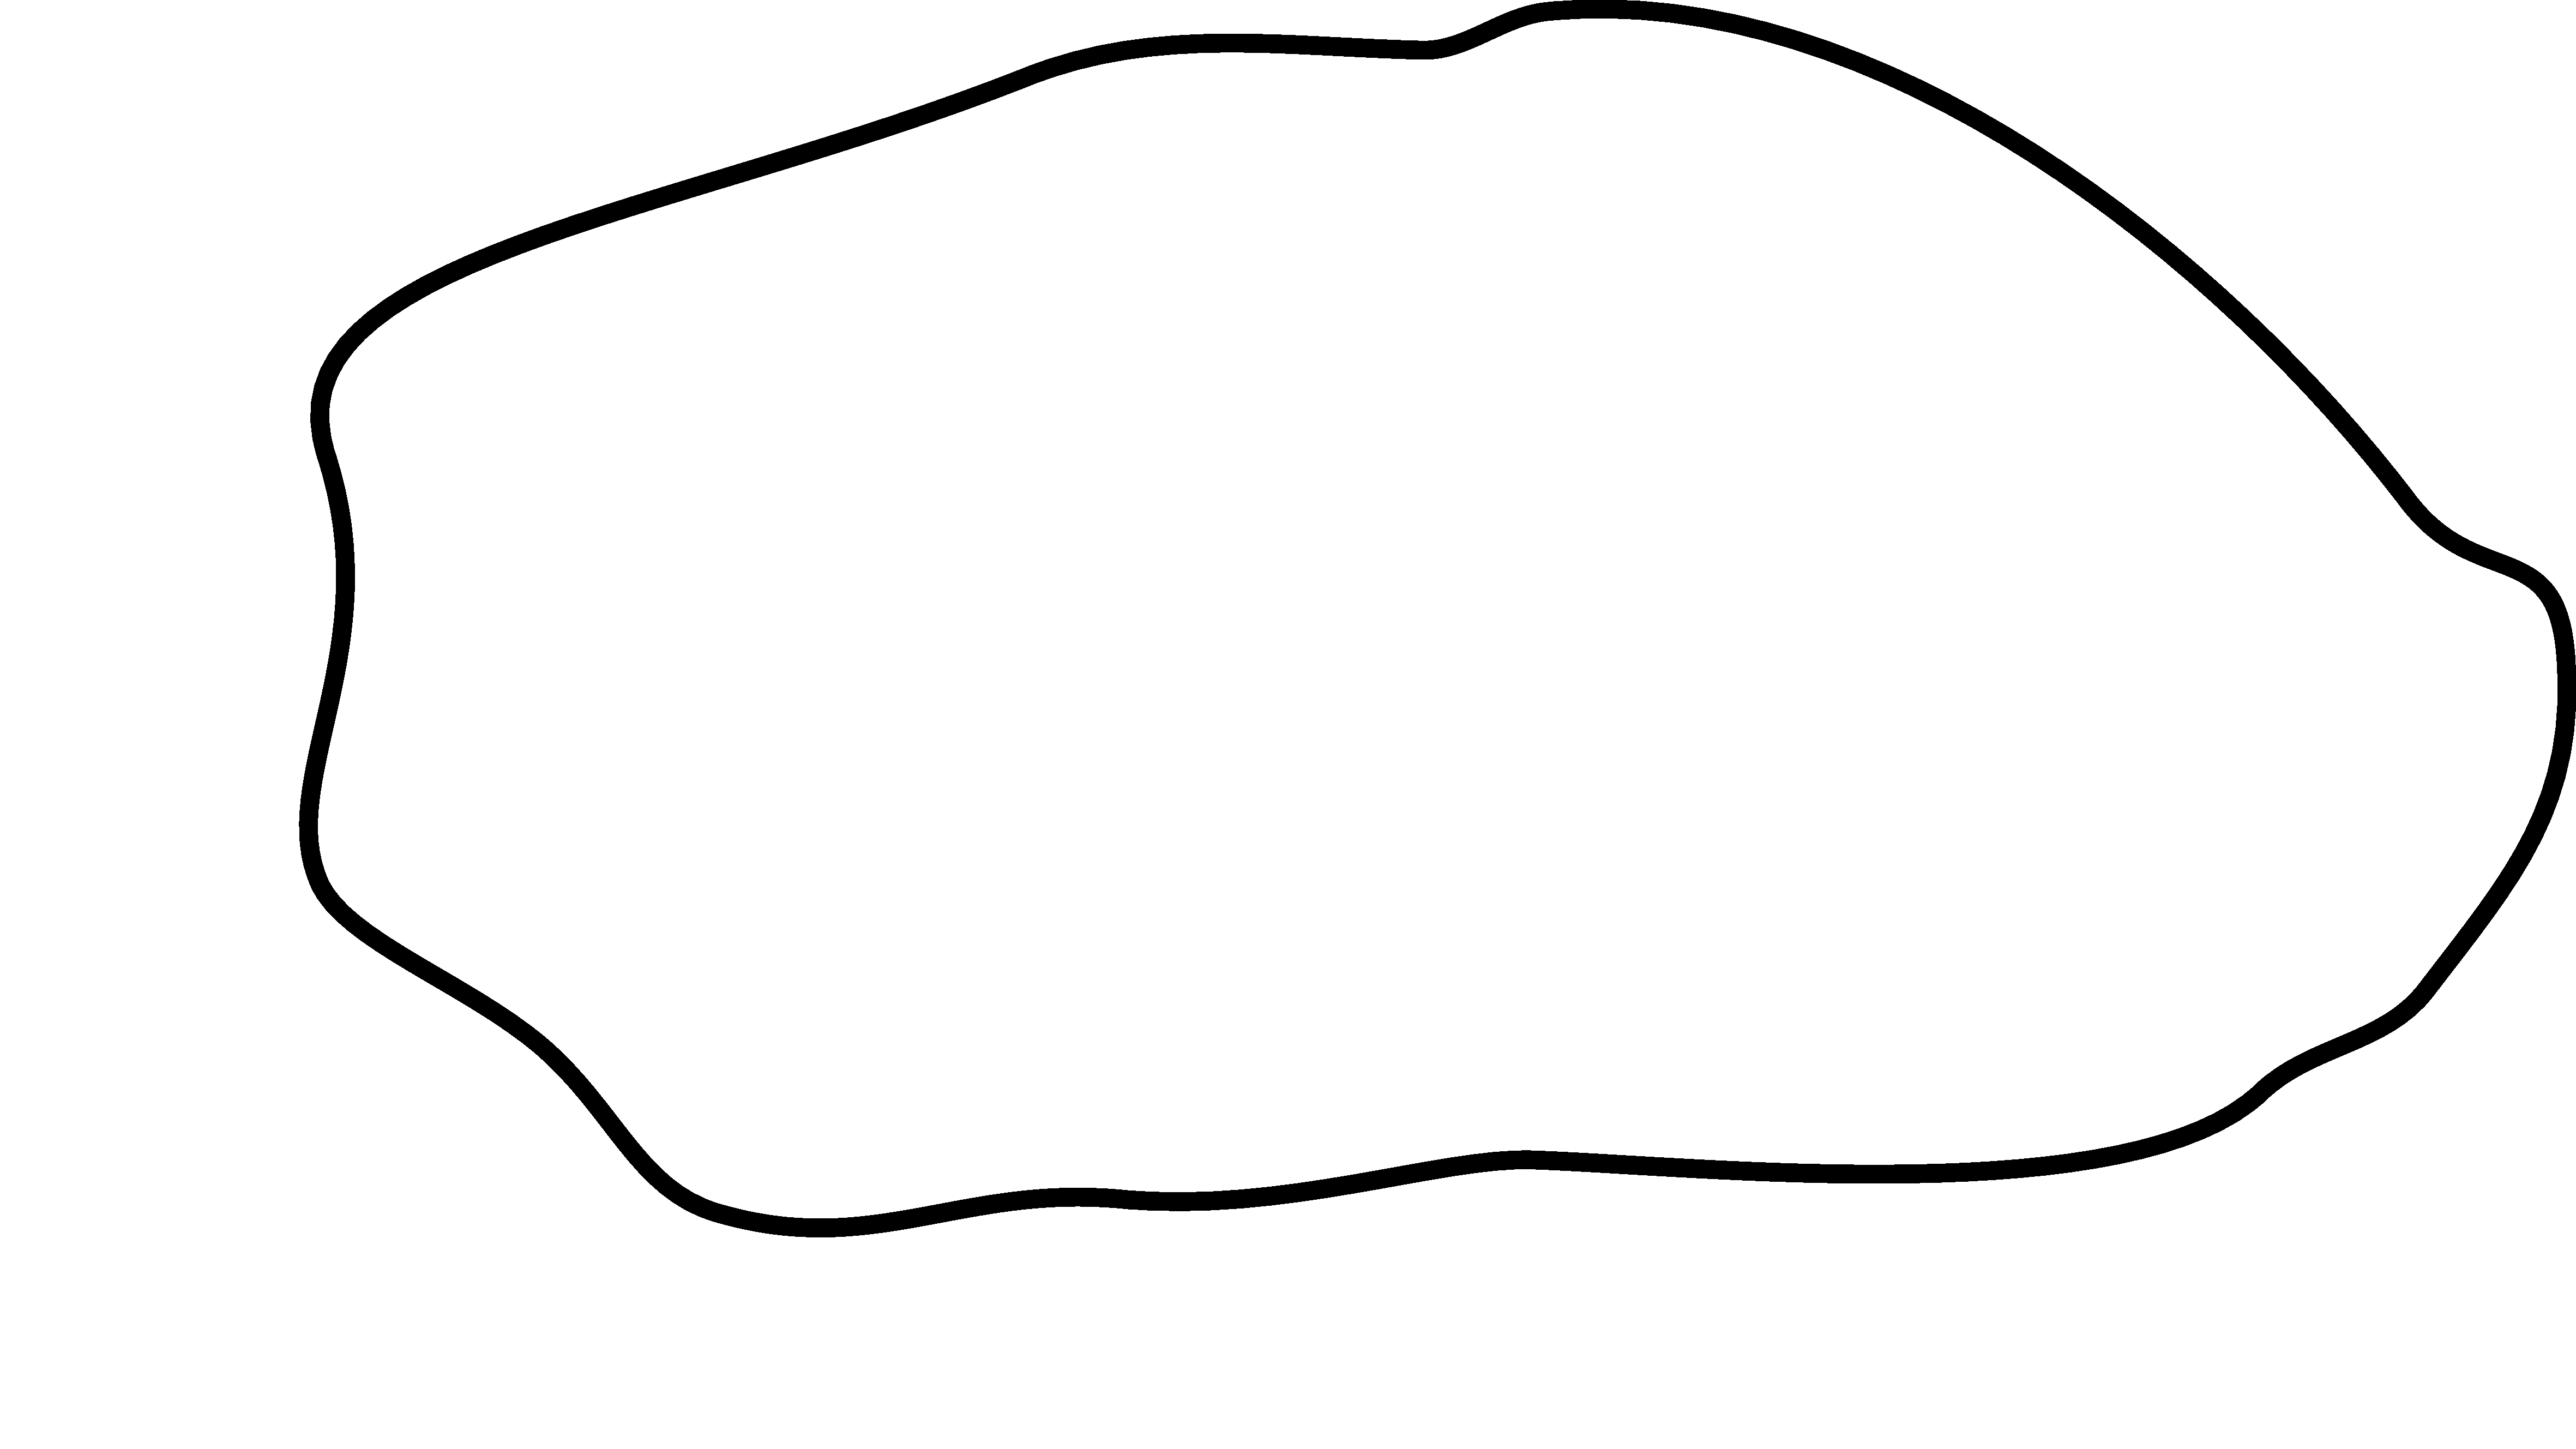
\includegraphics[height=45mm]{optainable_anal_optoutline}};
			\node< 4- 5> {
\includegraphics[height=45mm]{optainable_anal_asgdl_1}};
			\node< 6- 7> {
\includegraphics[height=45mm]{optainable_anal_asgdl_2}};
			\node< 8- 9> {
\includegraphics[height=45mm]{optainable_anal_asgdl_3}};
			\node<10-11> {
\includegraphics[height=45mm]{optainable_anal_asgdl_4}};
			\node<12-13> {
\includegraphics[height=45mm]{optainable_anal_asgdl_5}};
			\node<14-15> {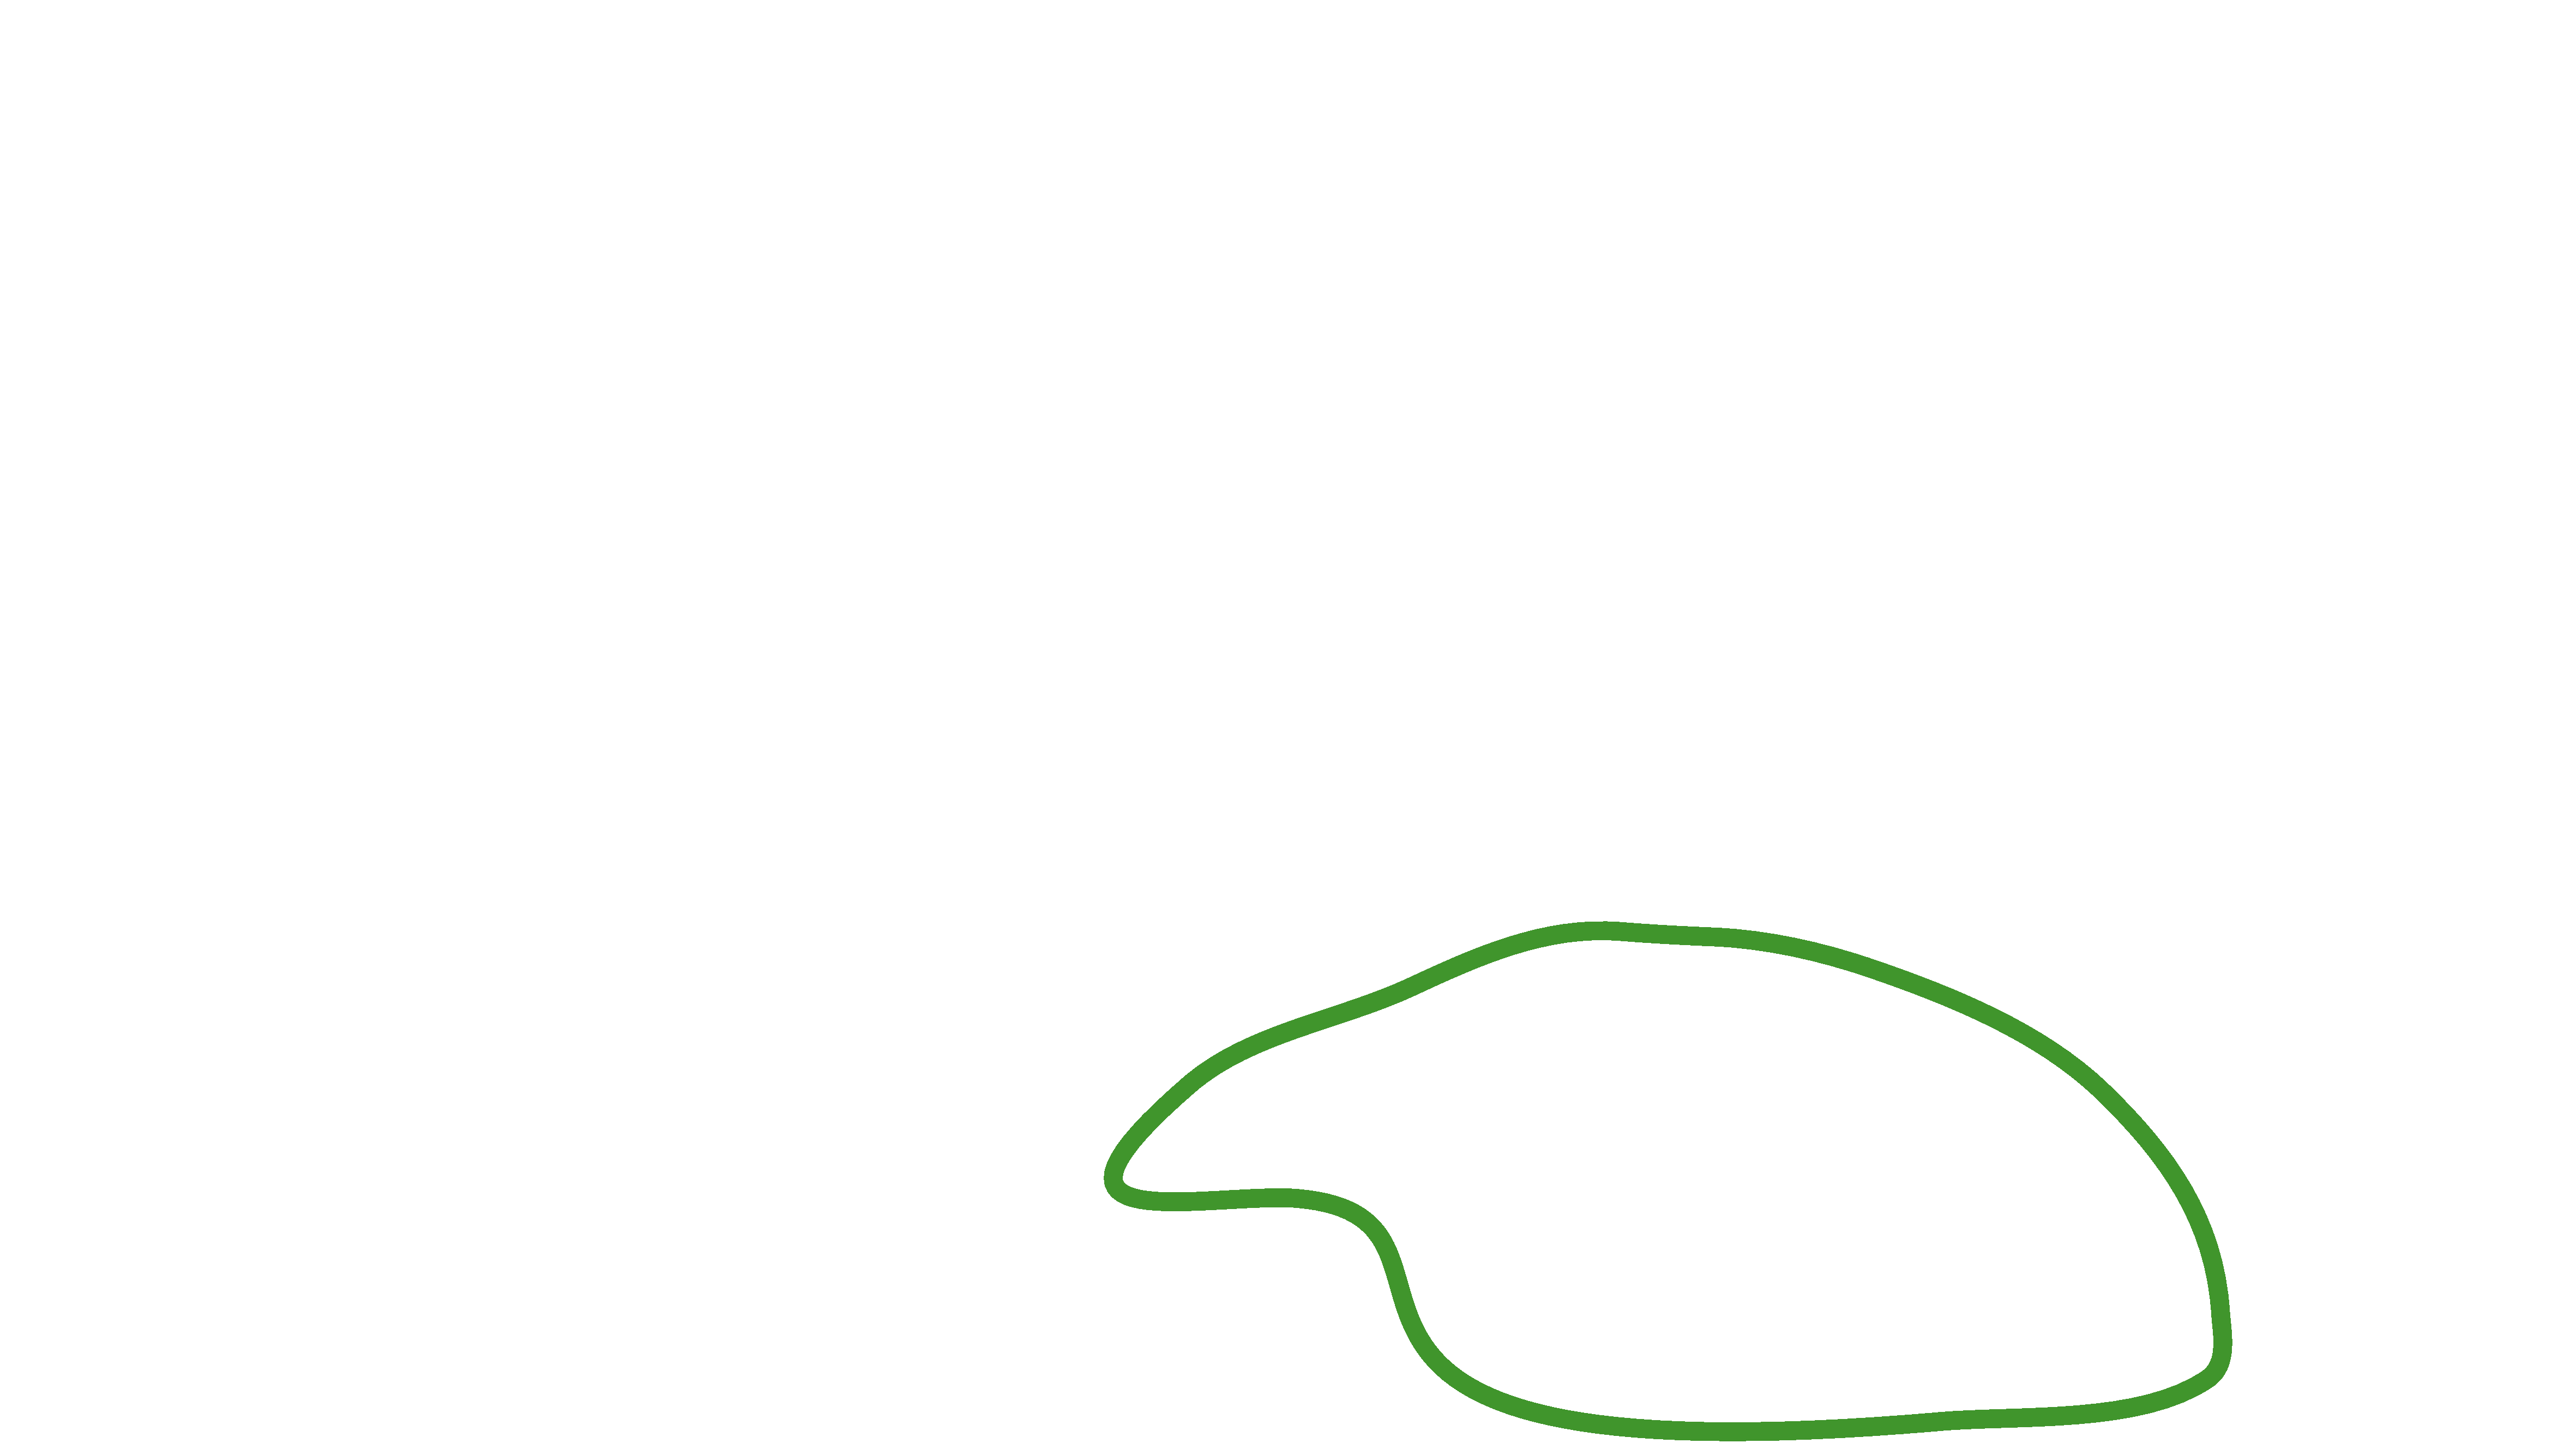
\includegraphics[height=45mm]{optainable_anal_asgdl_6}};
			\node<16-  > {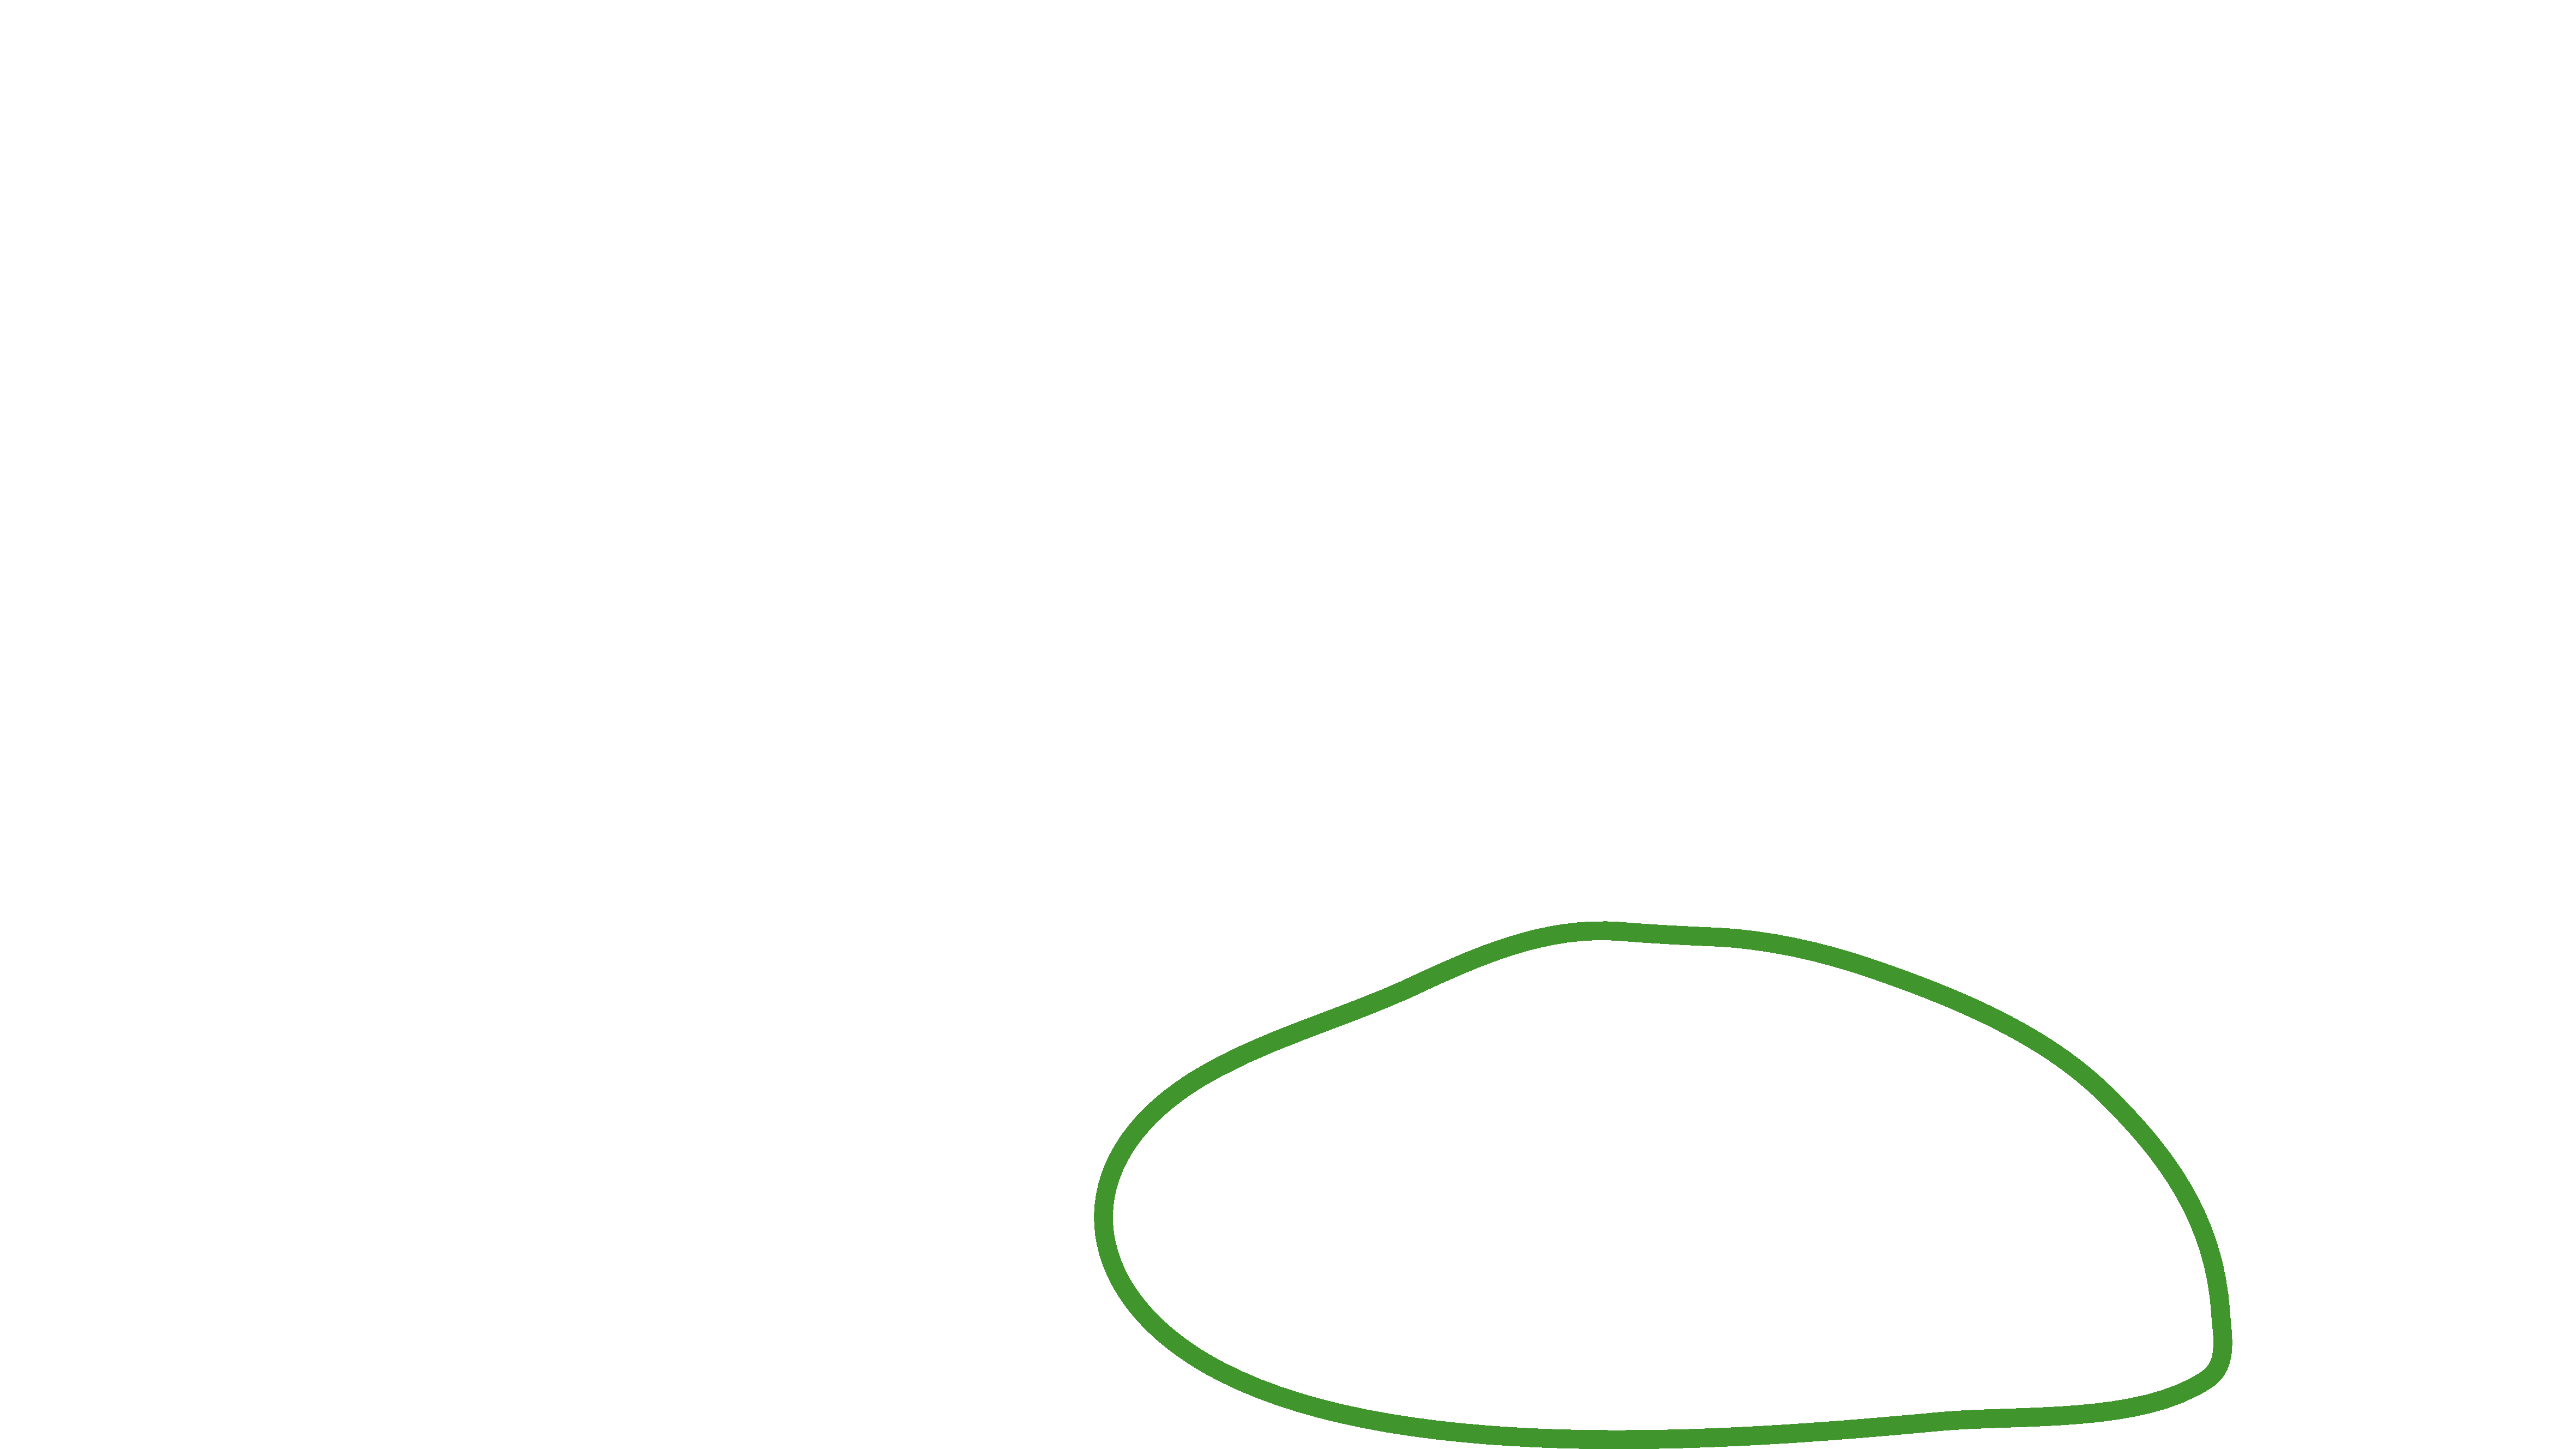
\includegraphics[height=45mm]{optainable_anal_asgdl_7}};
			\node< 5-  > {
\includegraphics[height=45mm]{optainable_anal_lost_1}};
			\node< 7-  > {
\includegraphics[height=45mm]{optainable_anal_lost_2}};
			\node< 9-  > {
\includegraphics[height=45mm]{optainable_anal_lost_3}};
			\node<11-  > {
\includegraphics[height=45mm]{optainable_anal_lost_4}};
			\node<13-  > {
\includegraphics[height=45mm]{optainable_anal_lost_5}};
			\node<15-  > {
\includegraphics[height=45mm]{optainable_anal_lost_6}};
			\node<17-  > {
\includegraphics[height=45mm]{optainable_anal_lost_7}};
			\node<23   > {
\includegraphics[height=45mm]{optainable_anal_emph_big}};
			\node<24   > {
\includegraphics[height=45mm]{optainable_anal_emph_small}};

			\node< 3->[legend             ] at (-3.5,  1.50) {\(\attopt{1}\)};
			\node< 4->[legend, dunkelgruen] at (-3.5,  0.75) {\(\alloc[\phaseii]\)};
			\node< 5->[legend, goetheblau ] at (-3.5, -0.00) {\(\lostset{l}\)};
			\node<18->[legend, dunkelgrau ] at (-3.5, -0.75) {\(\attopt{r}\)};
		\end{tikzpicture}
	\end{figure}
	\onslide*<30-38>{\beamerimage at (13cm, 3.25cm) {%
		\begin{minipage}[t][5cm]{0.4\textwidth}\begin{flalign*}
			\valuations[ \genericset[1] \given \genericset[2] ] \alt<36->{\le {}}{= {}}
			\onslide*<31-35>{&\valuations[\hairspace\genericitem[1] \given \genericset[2] ][\big]}
			\onslide*<32-35>{{} + {} \\ &\valuations[\hairspace\genericitem[2] \given \genericset[2] \cup \alertmath<35>{\braces[\big]{ \genericitem[1] }} ][\big]}
			\onslide*<33-35>{{} + {} \\ &\valuations[\hairspace\genericitem[3] \given \genericset[2] \cup \alertmath<35>{\braces[\big]{ \genericitem[1], \genericitem[2] }} ][\big]}
			\onslide*<34-35>{{} + {} \\ &\vdots}
			\onslide*<36   >{&\valuations[ \hairspace\genericitem[1] \given \genericset[2] ][\big] + {} \\ &\valuations[ \hairspace\genericitem[2] \given \genericset[2] ][\big] + {} \\ &\valuations[ \hairspace\genericitem[3] \given \genericset[2] ][\big] + {} \\ &\vdots}
			\onslide*<37-  >{\!\!\smashoperator{\sum_{\genericitem \in \genericset[1]}} \valuations[ \hairspace\genericitem  \given \genericset[2] ] }
			&&
		\end{flalign*}\end{minipage}
	};}
\end{frame}